\chapter{Příprava}
Pro provoz webové aplikace je zapotřebí backend server.
Pro tento účel jsem zvolil ICT centrum VŠB-TUO, kde jsem si nechal
vytvořit virtuální server.

\section{Operační systém a konfigurace DNS}
Jako operační systém serveru jsem zvolil Rocky Linux,
který mi byl doporučen administrátory školní sítě. Tato linuxová
distribuce je založena na RHEL. Součástí konfigurace VM je také
nastavení sítě. Neměnná IP adresa je získána z DHCP serveru,
avšak se jedná pouze o IPv4. IPv6 je potřeba nastavit ručně.
Pro server je předkonfigurovaný také DNS záznam pro IPv4 a IPv6,
který vypadá následovně:

\begin{verbatim}
Name                       Type   TTL   Section    IPAddress
----                       ----   ---   -------    ---------
pol0423-stu.vsb.cz         AAAA   7200  Answer     2001:718:1001:207::64
pol0423-stu.vsb.cz         A      7200  Answer     158.196.109.64
\end{verbatim}

DNS záznam AAAA je vazba na IPv6 adresu, zatímco DNS záznam A
je vazba na IPv4.

\section{Instalace OS a počáteční konfigurace serveru}
Server se nachází na VMware vSphere serveru, dostupný
na adrese vcs.vsb.cz. Prvním krokem byla instalace OS Rocky Linux,
která proběhla přes virtuální konzoli serveru. Instalační program
byl ve formě GUI, přes které jsem nastavil uživatelský účet správce
\texttt{marpolda}, nastavil jsem mu heslo a zapnul mu práva správce.
Účet správce \texttt{root} je vypnutý, lze ho tedy použít jen pomocí
příkazu \texttt{sudo}. Po instalaci OS byla dalším krokem instalace
nástrojů virtuálního stroje. Po neúspěšném pokusu v instalaci balíčku
VMware Tools jsem se rozhodl využít místo toho otevřený balíček
\texttt{open-vm-tools}. Pro práci s textovými soubory jsem si
také nainstaloval balíček \texttt{nano}, který poskytuje jednoduchý
textový editor přímo v příkazovém řádku.

\begin{figure}
    \centering
    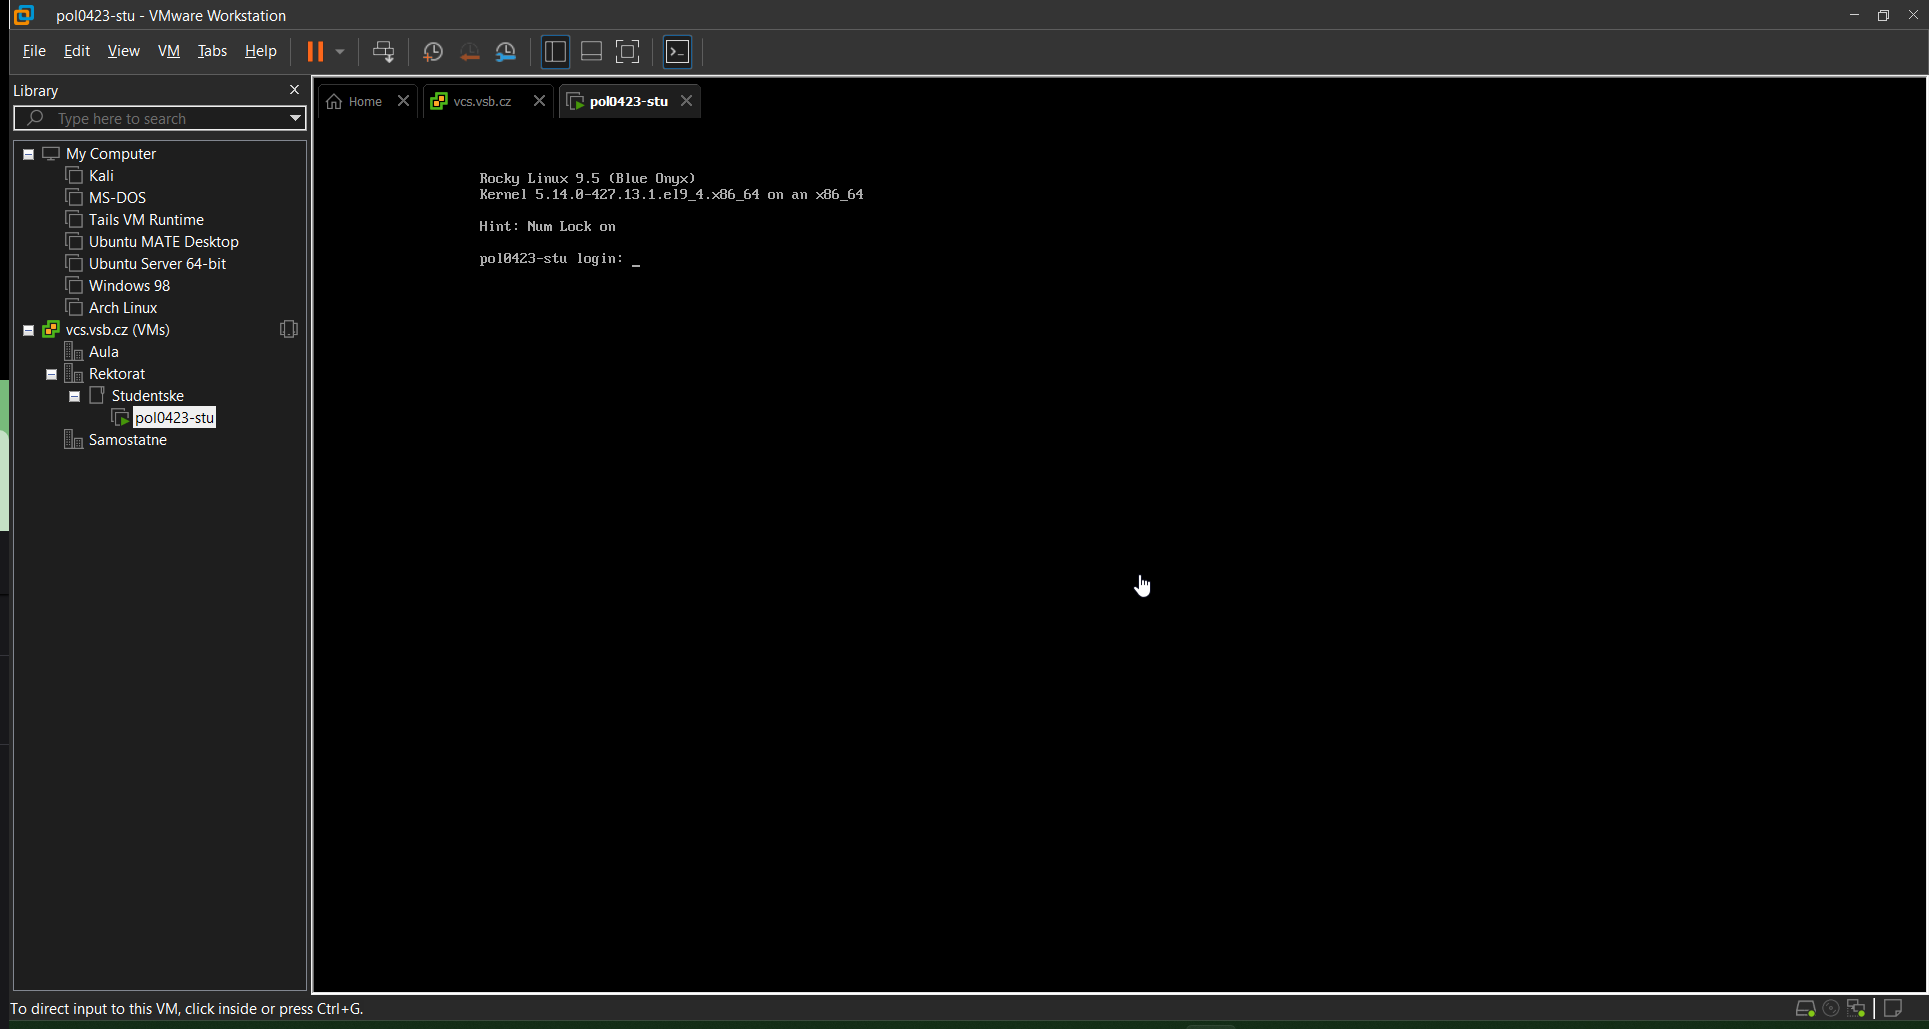
\includegraphics[width=0.75\linewidth]{Figures/vmware_console.png}
    \caption{Konzole virtuálního serveru ve VMware Workstation Pro}
    \label{fig:vmware-workstation-pro}
\end{figure}

Dalším krokem je nastavení IPv6 sítě. Jelikož IPv6 adresa není
DHCP serverem přidělena, je potřeba adresu nastavit ručně. Pro to
využijeme výše zmíněný DNS záznam pro IPv6 vazbu. Tento proces
je také zapotřebí provést pomocí virtuální konzole.

\begin{verbatim}
# ip a
1: lo: <LOOPBACK,UP,LOWER_UP> mtu 65536 qdisc noqueue state UNKNOWN
group default qlen 1000
    link/loopback 00:00:00:00:00:00 brd 00:00:00:00:00:00
    inet 127.0.0.1/8 scope host lo
       valid_lft forever preferred_lft forever
    inet6 ::1/128 scope host
       valid_lft forever preferred_lft forever
2: ens33: <BROADCAST,MULTICAST,UP,LOWER_UP> mtu 1500 qdisc fq_codel
state UP group default qlen 1000
    link/ether 00:50:56:ad:97:78 brd ff:ff:ff:ff:ff:ff
    altname enp2s1
    inet 158.196.109.64/24 brd 158.196.109.255 scope global dynamic
noprefixroute ens33
       valid_lft 55961sec preferred_lft 55961sec
    inet6 fe80::250:56ff:fead:9778/64 scope link noprefixroute
       valid_lft forever preferred_lft forever
# ip -6 addr add 2001:718:1001:207::64/64 dev ens33
# ip -6 route add default via 2001:718:1001:207::1 dev ens33
# ip a
1: lo: <LOOPBACK,UP,LOWER_UP> mtu 65536 qdisc noqueue state UNKNOWN
group default qlen 1000
    link/loopback 00:00:00:00:00:00 brd 00:00:00:00:00:00
    inet 127.0.0.1/8 scope host lo
       valid_lft forever preferred_lft forever
    inet6 ::1/128 scope host
       valid_lft forever preferred_lft forever
2: ens33: <BROADCAST,MULTICAST,UP,LOWER_UP> mtu 1500 qdisc fq_codel
state UP group default qlen 1000
    link/ether 00:50:56:ad:97:78 brd ff:ff:ff:ff:ff:ff
    altname enp2s1
    inet 158.196.109.64/24 brd 158.196.109.255 scope global dynamic
noprefixroute ens33
       valid_lft 55961sec preferred_lft 55961sec
    inet6 2001:718:1001:207::64/64 scope global
       valid_lft forever preferred_lft forever
    inet6 fe80::250:56ff:fead:9778/64 scope link noprefixroute
       valid_lft forever preferred_lft forever
\end{verbatim}

Otestujeme konektivitu IPv4 a IPv6:

\begin{verbatim}
PS C:\Users\marpo> ping -4 pol0423-stu.vsb.cz

Pinging pol0423-stu.vsb.cz [158.196.109.64] with 32 bytes of data:
Reply from 158.196.109.64: bytes=32 time<1ms TTL=61
Reply from 158.196.109.64: bytes=32 time<1ms TTL=61
Reply from 158.196.109.64: bytes=32 time<1ms TTL=61
Reply from 158.196.109.64: bytes=32 time<1ms TTL=61

Ping statistics for 158.196.109.64:
    Packets: Sent = 4, Received = 4, Lost = 0 (0% loss),
Approximate round trip times in milli-seconds:
    Minimum = 0ms, Maximum = 0ms, Average = 0ms
PS C:\Users\marpo> ping -6 pol0423-stu.vsb.cz

Pinging pol0423-stu.vsb.cz [2001:718:1001:207::64] with 32 bytes of data:
Reply from 2001:718:1001:207::64: time=2ms
Reply from 2001:718:1001:207::64: time=1ms
Reply from 2001:718:1001:207::64: time<1ms
Reply from 2001:718:1001:207::64: time=1ms

Ping statistics for 2001:718:1001:207::64:
    Packets: Sent = 4, Received = 4, Lost = 0 (0% loss),
Approximate round trip times in milli-seconds:
    Minimum = 0ms, Maximum = 2ms, Average = 1ms
\end{verbatim}

Pro přístup na server pomocí SSH jsem si také importoval ručně
přes konzoli SSH klíče obou mých počítačů, které využívají kvantově
rezistentní algoritmus \texttt{ed25519}. Z důvodu bezpečnosti jsem
také provedl vypnutí přihlašování pomocí uživatelského hesla.
Tento krok jsem provedl vytvořením nového souboru
\texttt{/etc/ssh/sshd\_config.d/01-nopasswordlogin.conf}
s následujícím obsahem:

\begin{verbatim}
#################################################
# Disable password logins
#################################################

PasswordAuthentication no
\end{verbatim}

Soubory v adresáři \texttt{/etc/ssh/sshd\_config.d} jsou automaticky
importovány v souboru\\
\texttt{/etc/ssh/sshd\_config}, který obsahuje konfiguraci SSH Daemon
serveru.

Následně stačilo restartovat službu SSH daemon:

\begin{verbatim}
# systemctl restart sshd.service
\end{verbatim}

Přístup na server pomocí SSH jsem následně otestoval:
\begin{verbatim}
PS C:\Users\marpo> ssh marpolda@pol0423-stu.vsb.cz
The authenticity of host 'pol0423-stu.vsb.cz (158.196.109.64)' can't be established.
ED25519 key fingerprint is SHA256:oHy0UKZisrWxLKQtp5Xpezo53FNXZudKJ6/WVHeScI4.
This host key is known by the following other names/addresses:
    ~/.ssh/known_hosts:18: 158.196.109.64
Are you sure you want to continue connecting (yes/no/[fingerprint])? yes
Warning: Permanently added 'pol0423-stu.vsb.cz' (ED25519) to the list of known hosts.
Enter passphrase for key 'C:\Users\marpo/.ssh/id_ed25519':
Last login: Sat Mar  1 14:01:55 2025 from 158.196.52.150
[marpolda@pol0423-stu ~]$
\end{verbatim}

Z mého druhého počítače jsem se také úspěšně přihlásil:
\begin{verbatim}
[marpolda@archlinuxx-laptop ~]$ ssh pol0423-stu.vsb.cz
Enter passphrase for key '/home/marpolda/.ssh/id_ed25519':
Last login: Sun Mar  2 19:21:04 2025 from 2001:718:1001:698:99e2:f1ff:4e67:7618
[marpolda@pol0423-stu ~]$
\end{verbatim}

Pro další práci, zejména s frontendem aplikace, se nám
bude hodit self-signed SSL certifikát. V reálném použití
bychom použili místo toho certifikační autoritu (např.
\emph{Let's Encrypt}), ale pro naše účely bude stačit
self-signed certifikát. Prohlížeči se to sice líbit
nebude, ale to není předmětem této práce.

Pro náš certifikát si nejdříve připravíme vhodné prostředí.
Certifikát vytvoříme pomocí uživatelského účtu \texttt{root}.
Příkazem \texttt{sudo bash} spustíme Bash v režimu účtu
\texttt{root}, a přesuneme se do adresáře \texttt{/etc/ssl}.
V něm vytvoříme nový adresář s názvem \texttt{self-signed},
a toto bude náš pracovní adresář.

\begin{verbatim}
[root@pol0423-stu ssl]# mkdir self-signed
[root@pol0423-stu ssl]# cd self-signed/
[root@pol0423-stu self-signed]# pwd
/etc/ssl/self-signed
\end{verbatim}

V tomto adresáři vytvoříme nový pár certifikátu a jeho
soukromého klíče. Oba soubory budou patřit účtu \texttt{root}.
K certifikátu vepíšeme údaje pro identifikaci certifikátu
(země původu, provincie, lokalita, název organizace, název
organizační jednotky, doména serveru a email správce).

\begin{verbatim}
[root@pol0423-stu self-signed]# openssl req -newkey rsa:4096
-x509  -sha512  -days 365 -nodes -out certificate.pem -keyout
privatekey.pem
..+.+...........+.+..+..........+......+.....+......+......+
.......+++++++++++++++++++++++++++++++++++++++++++++*..+.+
....................+...+.......+............+.....+.......
+.....+....+..+++++++++++++++++++++++++++++++++++++++++++++*
...+...+...+...........................+.........+......+.......
+................................+....+.....+.......+...+..+...+
......+.+..+..........+...........................+...+.........
......+............+...+...+++++
...+.+.....+......+...+....+.....+...+.......+........+...+....+
......+..+..................+.+.....+.+.....+.........+...+.......
+......+........+.......+..+.+.........+.....+.+......+.........+
.....+......+.+..+.......+..............+.+..............+....+...+
.....+.......+..+.............+.....+..........+...+..+.......+...
+++++++++++++++++++++++++++++++++++++++++++++*......+.+...+..+.+..
+...+.........+.........+.......+..+.+..+.............+.........+
.....+...+...+......+...+.+......+.........+.....+.........+......
+.+++++++++++++++++++++++++++++++++++++++++++++*.....+......+....+
........+...+....+...+.....+.+.....+...................+..+......+
.........+....+..............+++++
-----
You are about to be asked to enter information that will be incorporated
into your certificate request.
What you are about to enter is what is called a Distinguished Name or a DN.
There are quite a few fields but you can leave some blank
For some fields there will be a default value,
If you enter '.', the field will be left blank.
-----
Country Name (2 letter code) [XX]:CZ
State or Province Name (full name) []:Moravskoslezský kraj
Locality Name (eg, city) [Default City]:Ostrava
Organization Name (eg, company) [Default Company Ltd]:Vysoká škola
báňská - Technická univerzita Ostrava
Organizational Unit Name (eg, section) []:Fakulta elektrotechniky
a informatiky
Common Name (eg, your name or your server's hostname) []:pol0423-stu.vsb.cz
Email Address []:marek.polacek.st@vsb.cz
[root@pol0423-stu self-signed]# ll
total 8
-rw-r--r--. 1 root root 2464 Mar  3 17:05 certificate.pem
-rw-------. 1 root root 3272 Mar  3 17:04 privatekey.pem
\end{verbatim}

Obsah certifikátu si ověříme:
\begin{verbatim}
[root@pol0423-stu self-signed]# openssl x509 -noout -in
certificate.pem -text
Certificate:
    Data:
        Version: 3 (0x2)
        Serial Number:
            43:26:47:1f:c5:16:c6:8a:ef:7b:0f:52:17:3c:
28:a8:55:75:9b:c1
        Signature Algorithm: sha512WithRSAEncryption
        Issuer: C=CZ, ST=Moravskoslezský kraj, L=Ostrava,
O=Vysoká Å¡kola báÅská - Technická univerzita Ostrava,
OU=Fakulta elektrotechniky a informatiky, CN=pol0423-stu.vsb.cz,
emailAddress=marek.polacek.st@vsb.cz
        Validity
            Not Before: Mar  3 16:05:17 2025 GMT
            Not After : Mar  3 16:05:17 2026 GMT
        Subject: C=CZ, ST=Moravskoslezský kraj, L=Ostrava,
O=Vysoká Å¡kola báÅská - Technická univerzita Ostrava,
OU=Fakulta elektrotechniky a informatiky, CN=pol0423-stu.vsb.cz,
emailAddress=marek.polacek.st@vsb.cz
        Subject Public Key Info:
            Public Key Algorithm: rsaEncryption
                Public-Key: (4096 bit)
                Modulus:
                    00:c9:62:38:15:9d:07:f5:3e:3d:b2:38:53:28:72:
                    a6:8a:c4:34:2e:ba:71:0b:f3:9a:e3:2c:08:43:7d:
                    34:84:a0:14:38:e5:89:2b:01:05:b1:66:38:f5:08:
                    4b:2e:ac:87:42:bd:09:a6:97:1c:2b:b6:28:ab:4e:
                    9b:3c:f2:47:e1:37:3e:14:a8:ee:dc:91:4b:9e:23:
                    31:66:c6:49:35:b8:0c:c3:31:ee:e0:b1:96:3a:ed:
                    d1:b9:24:31:a3:79:8e:23:83:59:9d:54:50:3e:24:
                    52:b1:45:1f:24:b5:e3:40:30:b5:6c:92:fb:db:fa:
                    c8:9d:4d:e3:7a:c6:b1:76:9d:3f:d2:44:61:50:e0:
                    4f:2a:f5:b9:ee:5b:3c:56:02:24:39:91:d8:03:bf:
                    07:e2:b6:bd:bd:25:04:f5:8e:f4:c4:f4:dc:ef:36:
                    9f:9a:60:2f:7a:86:fb:03:3a:40:85:13:17:6b:1b:
                    2a:16:f2:8a:47:c5:78:2c:0a:eb:85:06:1f:7c:8b:
                    e5:c6:6a:fa:8a:3a:8e:47:a3:bb:25:74:e2:f5:13:
                    47:a1:6a:b9:9c:90:70:cc:71:b4:e9:1b:28:6e:f3:
                    2a:0a:31:f4:2d:b6:a6:35:5a:7b:65:28:1a:bf:0b:
                    4d:ca:4a:3b:4b:4f:71:e5:fc:a3:08:f0:41:52:94:
                    6e:cd:73:89:09:60:bc:29:2d:5e:a0:72:3a:b6:22:
                    c0:98:5e:df:8e:83:c8:a0:13:23:7d:a5:55:ec:bd:
                    91:2a:cf:68:52:1e:ec:ee:1a:db:ae:a4:da:19:e7:
                    a1:dd:91:5e:66:70:a8:f2:35:35:6c:24:c0:03:10:
                    48:a6:50:39:59:8e:fd:ee:51:40:ba:a3:b5:fb:44:
                    3a:0c:c1:be:87:8d:9b:82:ec:5a:c0:6d:cf:27:73:
                    32:9a:bb:cc:45:86:b6:46:6b:e2:21:e9:dc:4c:17:
                    06:3b:98:07:49:cc:71:b2:b6:c8:57:d6:dd:d9:7a:
                    95:b3:77:30:5c:d4:dc:a5:b7:07:e1:6e:7f:cd:23:
                    2a:61:a7:9d:f8:b7:cc:e5:3f:7e:75:e6:68:b3:18:
                    fe:29:f3:99:2e:11:f2:13:c0:d9:0b:0e:d8:eb:2c:
                    f4:bf:ee:98:0c:0a:56:c5:cd:12:6d:06:3d:17:99:
                    a6:a2:4b:16:6d:5f:51:90:b3:87:04:10:57:f8:54:
                    b6:dd:8d:9c:ed:e9:26:88:28:59:18:d6:94:b4:88:
                    8c:4d:3a:0f:a8:48:fb:44:1e:66:6e:b7:45:19:74:
                    69:d4:cb:ec:9e:67:79:e2:cf:3e:d2:d4:2c:15:e1:
                    b1:64:d2:76:a4:e1:e8:8f:df:90:2b:71:09:96:98:
                    46:78:d1
                Exponent: 65537 (0x10001)
        X509v3 extensions:
            X509v3 Subject Key Identifier:
                F2:41:E9:50:AC:72:59:5B:91:4A:C3:89:B7:30:5C:9E:
4E:2B:56:2A
            X509v3 Authority Key Identifier:
                F2:41:E9:50:AC:72:59:5B:91:4A:C3:89:B7:30:5C:9E:
4E:2B:56:2A
            X509v3 Basic Constraints: critical
                CA:TRUE
    Signature Algorithm: sha512WithRSAEncryption
    Signature Value:
        a9:ca:16:c1:fb:3d:3d:7c:d2:d0:d2:70:07:74:c2:3e:fb:6f:
        59:20:0e:b4:e2:9b:b6:41:02:94:ef:6d:f6:1d:f1:b6:83:8a:
        7e:aa:17:37:1e:30:f6:9d:26:f3:c7:6d:b2:c4:59:27:6a:b1:
        2f:e2:c5:c3:1d:fd:f2:81:fa:2e:27:51:5b:e3:be:ee:3a:40:
        fc:05:50:63:01:ab:b3:80:c1:a1:70:22:e3:8d:6f:2f:e4:e1:
        2d:89:15:c0:68:8b:9c:1c:5f:d6:6b:37:fb:06:53:61:fb:2d:
        94:af:36:e4:05:cc:8a:a3:92:d7:00:c0:26:19:6b:92:a8:ea:
        2a:15:44:87:dd:e5:73:3d:ed:dd:94:b0:47:a1:cd:b4:12:d1:
        5f:89:d7:73:48:5a:37:e3:e4:96:49:af:87:1c:b1:2a:bd:3f:
        6e:a5:33:fd:bc:84:55:81:c3:9d:54:c9:1b:d8:d0:c7:b9:60:
        27:a3:4d:e8:86:a4:2e:b2:07:8a:4d:d4:c2:f7:fb:19:16:c7:
        16:09:90:d5:e0:87:82:30:98:54:05:e3:4b:67:3d:e3:47:dd:
        1a:75:eb:95:df:80:0c:1b:c7:88:6e:1b:1f:10:49:bf:7f:06:
        2d:f1:1d:8a:59:54:8b:c0:9e:a8:a5:26:eb:4d:dd:b6:a9:af:
        63:b8:0f:19:cf:f1:54:62:29:18:23:9c:40:6d:57:bf:dc:52:
        4d:5b:fc:1b:90:75:17:e8:5b:a6:e4:3d:48:7a:59:29:d1:54:
        c4:18:91:db:c5:2d:dc:e4:4f:e5:ef:05:e4:ab:19:0e:6b:d6:
        7e:f5:24:91:3a:5c:9a:28:be:e8:20:dc:17:3b:06:57:99:48:
        0f:4e:0d:d6:0b:dc:7b:17:19:50:de:ca:81:fe:95:c1:f6:42:
        bc:b9:f4:bb:54:0e:01:e0:5f:38:7e:ec:e8:eb:33:24:de:cd:
        b6:71:cd:70:2e:d7:e6:43:69:b0:20:a6:dc:fd:43:dd:b4:97:
        c0:6f:0f:02:e6:ea:95:c8:f3:6e:8b:7d:d7:46:a3:cf:56:38:
        bd:c9:89:85:8c:df:73:6a:2f:6f:08:d2:e7:ac:86:c9:a5:69:
        41:79:2c:3c:1b:33:15:ff:d8:75:b5:15:5e:d4:4c:d3:a4:85:
        28:e2:b1:b3:03:e4:34:9d:37:22:68:8b:f3:f4:09:4c:01:4b:
        47:e2:5e:63:4e:19:b5:c3:d5:9f:b1:6e:7a:46:56:31:9e:77:
        ba:cc:b5:d1:df:a3:e6:82:06:7c:14:5a:2d:36:ee:ef:62:3e:
        f6:bc:8c:58:6c:a4:47:ca:06:8e:74:3e:1a:66:8a:67:b4:cd:
        3b:46:0d:f2:d5:f1:59:cf
\end{verbatim}

\section{Kontejnerizace a instalace služeb}
Nyní, když máme nastavený základní přístup, můžeme přistoupit
k instalaci softwaru pro kontejnerizaci a samotných kontejnerů
potřebných služeb. Pro kontejnerizaci jsem si vybral Docker,
který jsem nainstaloval z příslušného balíčku následovně:

\begin{verbatim}
# dnf install docker
\end{verbatim}

Dalším krokem je příprava samotných součástí aplikace. K tomu
jsem si vytvořil vývojové prostředí Gitu, ve kterém bude
probíhat vývoj aplikace a příprava pro její nasazení na server.
Toto prostředí se také nachází na GitHubu, kde je vidět
aktuální podoba této aplikace. Aplikaci jsem se rozhodl pojmenovat
\emph{PetrolScan}. Všechny součásti aplikace obsahují soubor
\texttt{Dockerfile}, který vytváří Docker obrázek dané součásti.
Všechny tyto součásti jsou pospojovány souborem \texttt{docker-compose.yml},
který součásti propojuje a vytváří tak ucelenou službu.

Vyvíjené součásti aplikace jsou:

\begin{itemize}
    \item Webová aplikace:
        \texttt{\url{https://github.com/POL0423/petrolscan-web-app}}
    \item Crawler:
        \texttt{\url{https://github.com/POL0423/petrolscan-crawler}}
    \item Docker Compose:
        \texttt{\url{https://github.com/POL0423/petrolscan-docker-compose}}
\end{itemize}

\subsection{Výběr softwaru}

Jako první jsem se rozhodl najít vhodné self-hosted webové crawlery
a scrapery. Na dotaz k vyhledávání mi ChatGPT našlo následující možnosti:

\begin{itemize}
    \item Crawlee
    \item Scrapy
    \item EasySpider
\end{itemize}

\subsubsection{Crawlee}

Tento crawler funguje v Node.js, a nabízí jednoduchou instalaci pomocí
jednoduchého příkazu. Zkušební test ukázkového crawleru proběhl v pořádku.
První pokus o spuštění neuspěl, neboť chyběly Playwright bezhlavičkové
prohlížeče. Po instalaci těchto prohlížečů se již crawler spustil.

\begin{verbatim}
$ npx crawlee create test-crawler
Need to install the following packages:
crawlee@3.13.0
Ok to proceed? (y) y
npm WARN deprecated lodash.isequal@4.5.0: This package is deprecated.
Use require('node:util').isDeepStrictEqual instead.
? Please select the template for your new Crawlee project Getting started
example [TypeScript]
npm WARN deprecated lodash.isequal@4.5.0: This package is deprecated. Use
require('node:util').isDeepStrictEqual instead.

added 309 packages, and audited 310 packages in 12s

81 packages are looking for funding
  run `npm fund` for details

found 0 vulnerabilities
Project test-crawler was created. To run it, run "cd test-crawler" and
"npm start".
$ cd test-crawler/
$ npm start

> test-crawler@0.0.1 start
> npm run start:dev


> test-crawler@0.0.1 start:dev
> tsx src/main.ts

INFO  PlaywrightCrawler: Starting the crawler.
INFO  PlaywrightCrawler: Final request statistics: {"requestsFinished":0,
"requestsFailed":0,"retryHistogram":[],"requestAvgFailedDurationMillis":
null,"requestAvgFinishedDuration
Millis":null,"requestsFinishedPerMinute":0,"requestsFailedPerMinute":0,
"requestTotalDurationMillis":0,"requestsTotal":0,"crawlerRuntimeMillis":685}
INFO  PlaywrightCrawler: Finished! Total 0 requests: 0 succeeded, 0 failed.
{"terminal":true}
node:internal/process/esm_loader:34
      internalBinding('errors').triggerUncaughtException(
                                ^

Failed to launch browser. Please check the following:
- Try installing the required dependencies by running `npx playwright
install --with-deps` (https://playwright.dev/docs/browsers).
[...]
$ npx playwright install
Downloading Chromium 134.0.6998.35 (playwright build v1161) from ...
141.8 MiB [====================] 100% 0.0s
Chromium 134.0.6998.35 (playwright build v1161) downloaded to ...
Downloading Chromium Headless Shell 134.0.6998.35 (playwright build v1161)
from ...
87.8 MiB [====================] 100% 0.0s
Chromium Headless Shell 134.0.6998.35 (playwright build v1161) downloaded
to ...
Downloading Firefox 135.0 (playwright build v1475) from ...
91.5 MiB [====================] 100% 0.0s
Firefox 135.0 (playwright build v1475) downloaded to ...
Downloading Webkit 18.4 (playwright build v2140) from ...
52.8 MiB [====================] 100% 0.0s
Webkit 18.4 (playwright build v2140) downloaded to ...
Downloading FFMPEG playwright build v1011 from ...
1.3 MiB [====================] 100% 0.0s
FFMPEG playwright build v1011 downloaded to ...
Downloading Winldd playwright build v1007 from ...
0.1 MiB [====================] 100% 0.0s
Winldd playwright build v1007 downloaded to ...
$ npm start

> test-crawler@0.0.1 start
> npm run start:dev


> test-crawler@0.0.1 start:dev
> tsx src/main.ts

INFO  PlaywrightCrawler: Starting the crawler.
INFO  PlaywrightCrawler: Title of https://crawlee.dev/ is 'Crawlee · Build
reliable crawlers. Fast.'
INFO  PlaywrightCrawler: Title of https://crawlee.dev/docs/examples is
'Examples | Crawlee · Build reliable crawlers. Fast.'
INFO  PlaywrightCrawler: Title of https://crawlee.dev/docs/quick-start is
'Quick Start | Crawlee · Build reliable crawlers. Fast.'
INFO  PlaywrightCrawler: Title of https://crawlee.dev/api/core is
'@crawlee/core | API | Crawlee · Build reliable crawlers. Fast.'
INFO  PlaywrightCrawler: Title of https://crawlee.dev/api/core/changelog
is 'Changelog | API | Crawlee · Build reliable crawlers. Fast.'
INFO  PlaywrightCrawler: Title of https://crawlee.dev/blog is 'Crawlee
Blog - learn how to build better scrapers | Crawlee · Build reliable
crawlers. Fast.'
INFO  PlaywrightCrawler: Title of https://crawlee.dev/python is 'Crawlee
for Python · Fast, reliable Python web crawlers.'
INFO  PlaywrightCrawler: Title of https://crawlee.dev/docs/next/quick-
start is 'Quick Start | Crawlee · Build reliable crawlers. Fast.'
INFO  PlaywrightCrawler: Title of https://crawlee.dev/docs/3.12/quick-
start is 'Quick Start | Crawlee · Build reliable crawlers. Fast.'
INFO  PlaywrightCrawler: Title of https://crawlee.dev/docs/3.10/quick-
start is 'Quick Start | Crawlee · Build reliable crawlers. Fast.'
INFO  PlaywrightCrawler: Title of https://crawlee.dev/docs/3.11/quick-
start is 'Quick Start | Crawlee · Build reliable crawlers. Fast.'
INFO  PlaywrightCrawler: Title of https://crawlee.dev/docs/3.9/quick-
start is 'Quick Start | Crawlee · Build reliable crawlers. Fast.'
INFO  PlaywrightCrawler: Title of https://crawlee.dev/docs/3.8/quick-
start is 'Quick Start | Crawlee · Build reliable crawlers. Fast.'
INFO  PlaywrightCrawler: Title of https://crawlee.dev/docs/3.7/quick-
start is 'Quick Start | Crawlee · Build reliable crawlers. Fast.'
INFO  PlaywrightCrawler: Title of https://crawlee.dev/docs/3.3/quick-
start is 'Crawlee · Build reliable crawlers. Fast.'
INFO  PlaywrightCrawler: Title of https://crawlee.dev/docs/3.4/quick-
start is 'Quick Start | Crawlee · Build reliable crawlers. Fast.'
INFO  PlaywrightCrawler: Title of https://crawlee.dev/docs/3.6/quick-
start is 'Quick Start | Crawlee · Build reliable crawlers. Fast.'
INFO  PlaywrightCrawler: Title of https://crawlee.dev/docs/3.5/quick-
start is 'Quick Start | Crawlee · Build reliable crawlers. Fast.'
INFO  PlaywrightCrawler: Title of https://crawlee.dev/docs/3.2/quick-
start is 'Quick Start | Crawlee · Build reliable crawlers. Fast.'
INFO  PlaywrightCrawler: Title of https://crawlee.dev/docs/3.0/quick-
start is 'Quick Start | Crawlee · Build reliable crawlers. Fast.'
INFO  PlaywrightCrawler: Title of https://crawlee.dev/docs/3.1/quick-
start is 'Quick Start | Crawlee · Build reliable crawlers. Fast.'
INFO  PlaywrightCrawler: Title of https://crawlee.dev/docs/introduction
is 'Introduction | Crawlee · Build reliable crawlers. Fast.'
INFO  PlaywrightCrawler: Title of https://crawlee.dev/docs/guides/
javascript-rendering is 'JavaScript rendering | Crawlee · Build reliable
crawlers. Fast.'
INFO  PlaywrightCrawler: Crawler reached the maxRequestsPerCrawl limit
of 20 requests and will shut down soon. Requests that are in progress
will be allowed to finish.
INFO  PlaywrightCrawler: Earlier, the crawler reached the
maxRequestsPerCrawl limit of 20 requests and all requests that were in
progress at that time have now finished. In total, the crawler processed
23 requests and will shut down.
INFO  PlaywrightCrawler: Final request statistics: {"requestsFinished":23,
"requestsFailed":0,"retryHistogram":[23],"requestAvgFailedDurationMillis":
null,"requestAvgFinishedDurationMillis":3071,"requestsFinishedPerMinute":
45,"requestsFailedPerMinute":0,"requestTotalDurationMillis":70640,
"requestsTotal":23,"crawlerRuntimeMillis":30383}
INFO  PlaywrightCrawler: Finished! Total 23 requests: 23 succeeded,
0 failed. {"terminal":true}
\end{verbatim}

Velmi příjemným zjištěním bylo, že builder již automaticky vygeneruje
soubor \texttt{Dockerfile}, pro crawler tak lze rovnou vytvořit
Docker image, který se jen posléze nahraje na Docker Hub a lze s ním
dále pracovat.

\subsubsection{Scrapy}

% TODO: Projít Scrapy a k tomu přidruženou dokumentaci.

\subsubsection{EasySpider}

% TODO: Projít EasySpider a k tomu přidruženou dokumentaci.

\subsubsection{Konečný verdikt}

% TODO: Vybrat vhodný software

\subsection{Databáze}

% TODO: Databázové systémy

\subsection{Frontend}

% TODO: Tvorba frontendu

\endinput
